\pdfinfoomitdate=1
\pdftrailerid{}
\documentclass[12pt]{article}
\usepackage[letterpaper,margin=0.65in,headheight=16pt,headsep=18pt,footskip=25pt]{geometry}
\usepackage{tikz,amsmath,array,fancyhdr}
\usepackage[T1]{fontenc}
\usepackage{lmodern}
\renewcommand{\familydefault}{\sfdefault}
\pagestyle{fancy}\fancyhf{}
\newcommand{\band}{Grades 3--5}
\fancyhead[L]{\small Week 93 / Squaring a rectangle / \band}
\fancyfoot[L]{\footnotesize Bellingham Math Circle / Week 93 / W93-S-v3}
\fancyfoot[R]{\footnotesize\thepage}
\renewcommand{\headrulewidth}{0.4pt}\renewcommand{\footrulewidth}{0.4pt}
\setlength{\parindent}{0pt}\setlength{\parskip}{9pt}
\newcommand{\problem}[2]{\par\textbf{Problem #1:} #2\par}
\newcommand{\unitrect}[5]{% x,y,width,height,label
  \begin{scope}[shift={(#1,#2)}]
  \draw[step=1,gray!45,very thin] (0,0) grid (#3,#4);
  \draw[thick] (0,0) rectangle (#3,#4);
  \node[below] at (#3/2,0) {#3};
  \node[left] at (0,#4/2) {#4};
  \node[above] at (#3/2,#4) {#5};
  \end{scope}}
\begin{document}
Each grid-square edge is 1 unit. Rectangles turned around count as the same rectangle.

\problem{1}{Use all 24 square tiles to make each different rectangle you can. Draw your collection. Which rectangle comes closest to being a square? How long would the side of a square with the area of 24 tiles be?}

\vspace{3mm}
\begin{center}
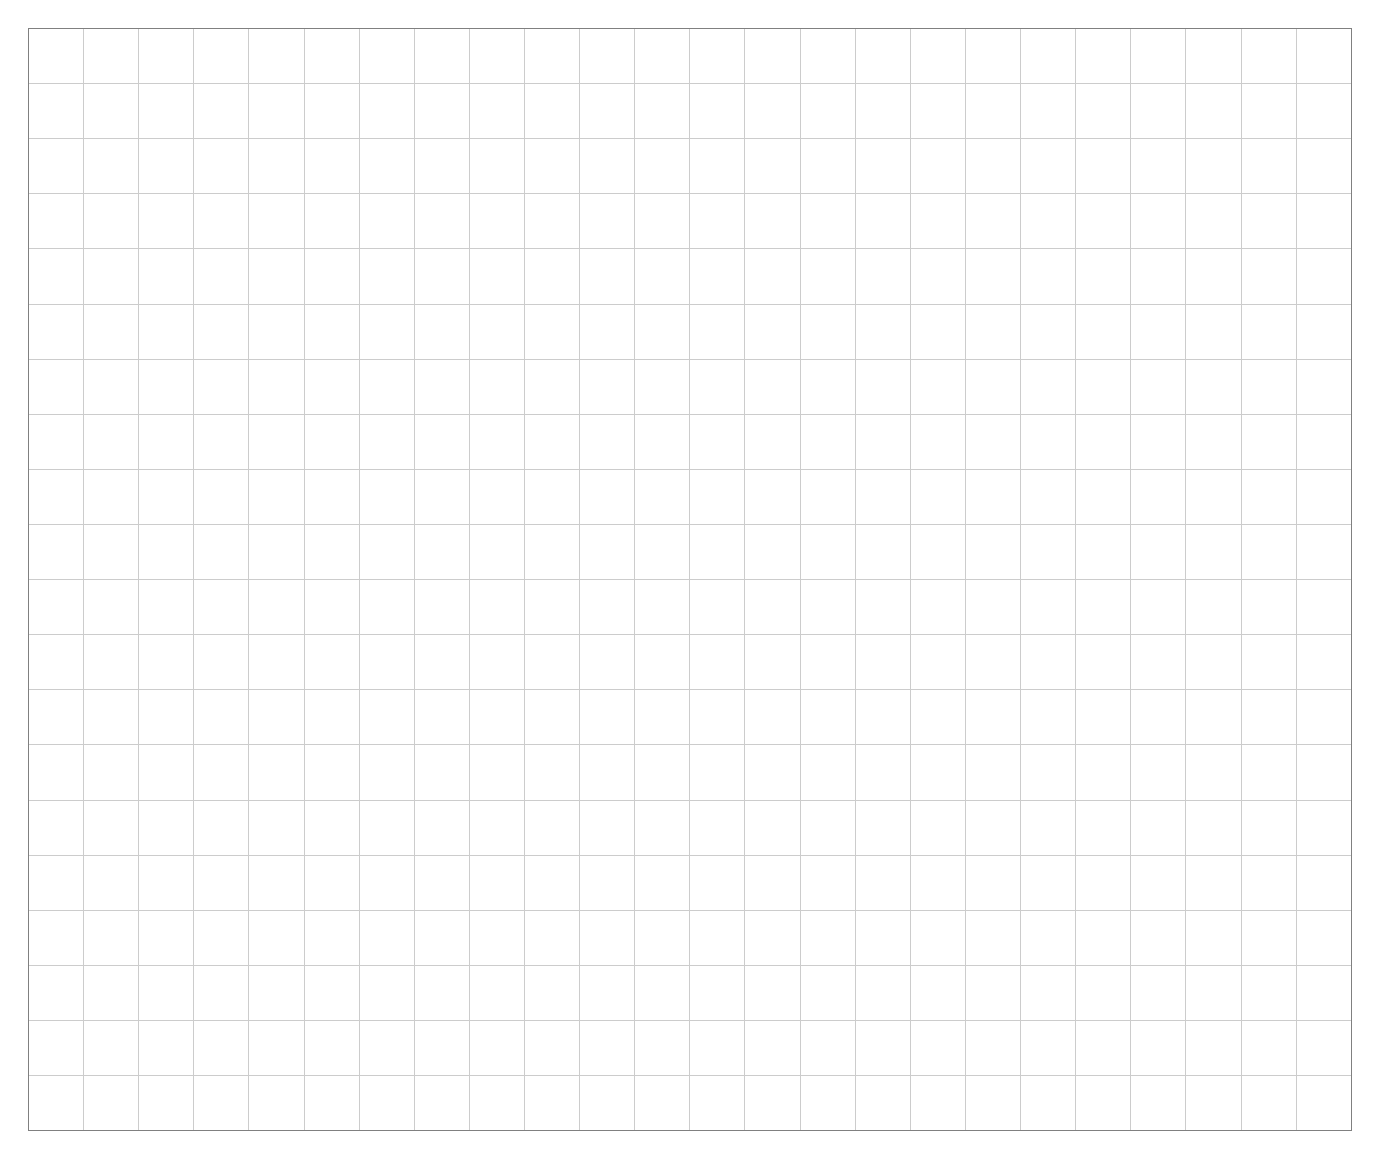
\begin{tikzpicture}[x=0.7cm,y=0.7cm]
\draw[step=1,gray!40,very thin] (0,0) grid (24,20);
\draw[gray] (0,0) rectangle (24,20);
\end{tikzpicture}
\end{center}
\vfill

\newpage

\problem{2}{Cut each rectangle into pieces and fit all its pieces inside the matching square, without overlaps. Can the uncovered part be a single square, of any size, in each case? Find its side length.}

\begin{center}
\begin{tikzpicture}[x=1.5cm,y=1.5cm]
\unitrect{0}{6}{6}{2}{A}
\unitrect{7}{5}{4}{4}{A}
\unitrect{0}{0.5}{4}{2}{B}
\unitrect{7}{0}{3}{3}{B}
\unitrect{0}{-3.5}{5}{1}{C}
\unitrect{7}{-4.5}{3}{3}{C}
\end{tikzpicture}
\end{center}
\vfill

\newpage

A reshaping move keeps the area: average the two sides, then divide the area by that average to get the other new side.

\begin{center}
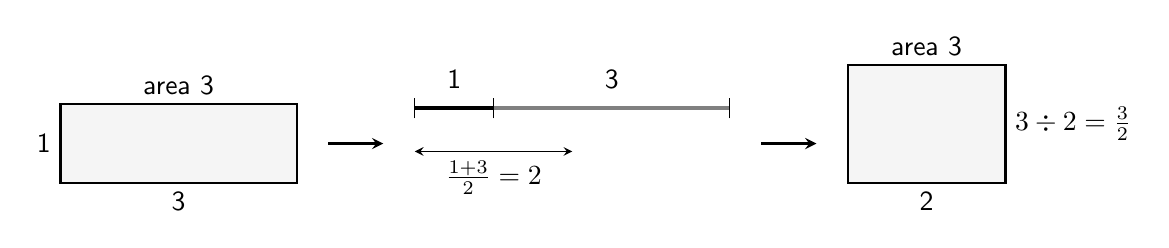
\begin{tikzpicture}[x=1cm,y=1cm,>=stealth]
\draw[thick,fill=gray!8] (0,0) rectangle (3,1);
\node[below] at (1.5,0) {3};\node[left] at (0,.5) {1};
\node[above] at (1.5,1) {area 3};
\draw[->,thick] (3.4,.5)--(4.1,.5);
\draw[very thick] (4.5,.95)--(5.5,.95);
\draw[very thick,gray] (5.5,.95)--(8.5,.95);
\foreach \x in {4.5,5.5,8.5} \draw (\x,.82)--(\x,1.08);
\node[above] at (5,1.08) {1};\node[above] at (7,1.08) {3};
\draw[<->] (4.5,.4)--(6.5,.4);
\node[below] at (5.5,.4) {$\frac{1+3}{2}=2$};
\draw[->,thick] (8.9,.5)--(9.6,.5);
\draw[thick,fill=gray!8] (10,0) rectangle (12,1.5);
\node[below] at (11,0) {2};\node[right] at (12,.75) {$3\div2=\frac32$};
\node[above] at (11,1.5) {area 3};
\end{tikzpicture}
\end{center}

Write each side length exactly, using fractions when needed.

\problem{3}{Reshape each rectangle once. Mark the old and new side lengths on its number line. Which two of those four lengths give the tightest guaranteed range for the side of a square with that area?}

\begin{center}
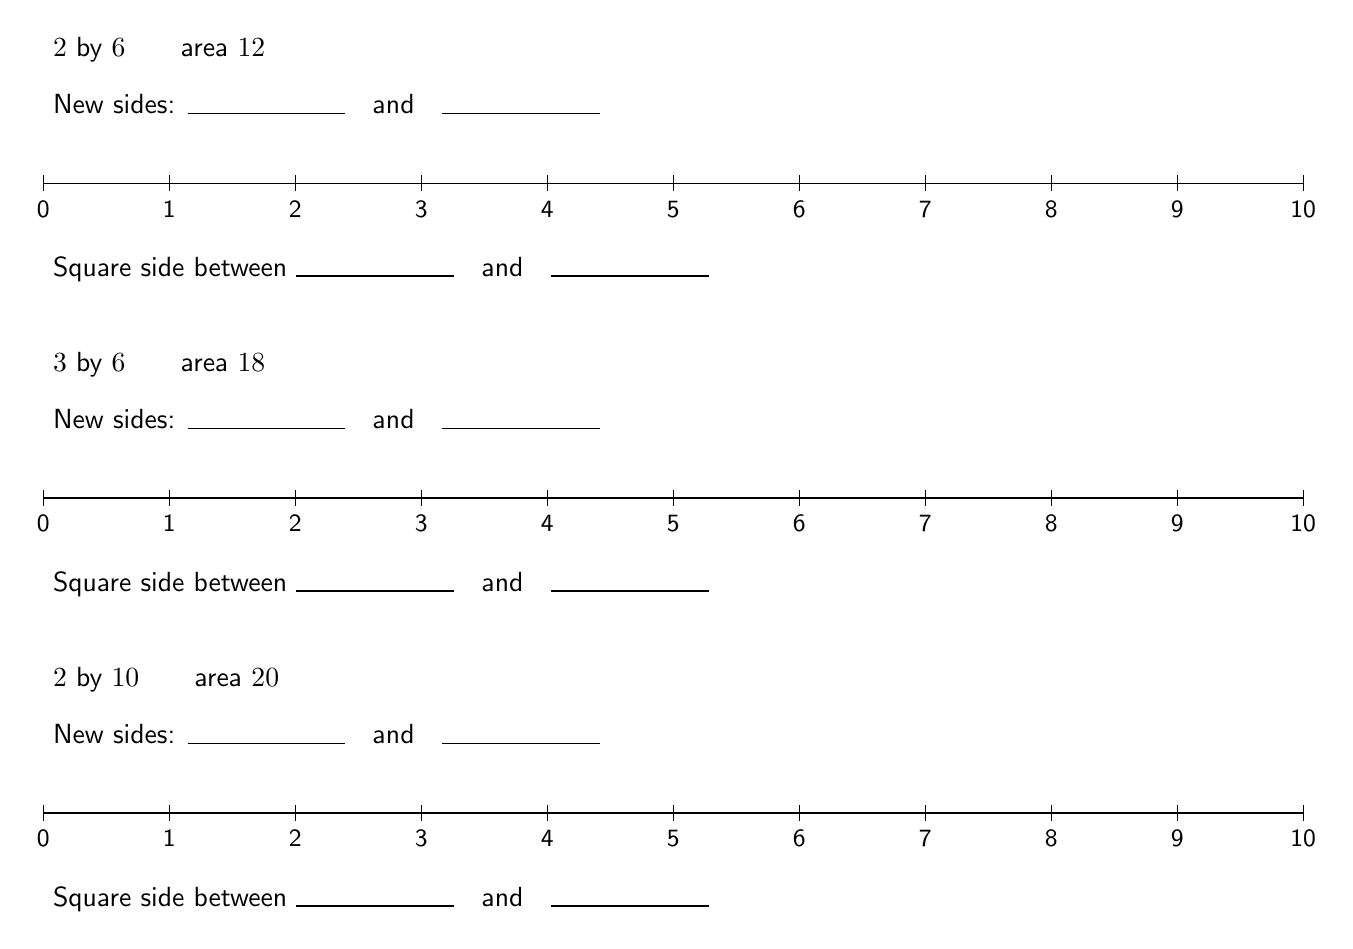
\begin{tikzpicture}[x=1cm,y=1cm]
\foreach \y/\a/\b/\area in {0/2/6/12,-4/3/6/18,-8/2/10/20} {
\node[anchor=west] at (0,\y) {$\a\ \text{by}\ \b\qquad\text{area }\area$};
\node[anchor=west] at (0,\y-.7) {New sides: \rule{2.0cm}{.4pt}\quad and\quad\rule{2.0cm}{.4pt}};
\draw (0,\y-1.7)--(16,\y-1.7);
\foreach \n in {0,...,10} {
\draw (1.6*\n,\y-1.6)--(1.6*\n,\y-1.8);
\node[below,font=\small] at (1.6*\n,\y-1.8) {\n};}
\node[anchor=west] at (0,\y-2.8) {Square side between \rule{2.0cm}{.4pt}\quad and\quad\rule{2.0cm}{.4pt}};
}
\end{tikzpicture}
\end{center}

\newpage

\problem{4}{Cut out the four cards from a spare copy of this page. They show four stages of reshaping one rectangle, with exact side lengths. Put them in order so each card follows from one reshaping move. Which card gives the tightest guaranteed range for the side of a square of area 12? Show why that square's side cannot lie outside your range.}

\begin{center}
\begin{tikzpicture}[x=1cm,y=1cm]
\draw (0,0) rectangle (7,2);\node at (.5,1.5) {A};\node at (3.5,1) {$\dfrac{24}{7}\quad\text{by}\quad\dfrac72$};
\draw (8,0) rectangle (15,2);\node at (8.5,1.5) {B};\node at (11.5,1) {$2\quad\text{by}\quad6$};
\draw (0,-2.5) rectangle (7,-.5);\node at (.5,-1) {C};\node at (3.5,-1.5) {$\dfrac{336}{97}\quad\text{by}\quad\dfrac{97}{28}$};
\draw (8,-2.5) rectangle (15,-.5);\node at (8.5,-1) {D};\node at (11.5,-1.5) {$3\quad\text{by}\quad4$};
\end{tikzpicture}
\end{center}
\vspace{29mm}

\problem{5}{Find two decimals one hundredth apart that trap the side of the square of area 12. Could either decimal be the exact side length? Give exact area checks for your answer.}

\vfill

\newpage

\renewcommand{\band}{Grades 4--5, ready for general reasoning}

\problem{6}{For any rectangle, is the square whose side is the average of the rectangle's sides always at least as large in area? Explain with a cut-and-rearrange picture. How much extra area does the square have?}

\begin{center}
\begin{tikzpicture}[x=1cm,y=1cm]
\draw[thick] (0,0) rectangle (7,3);
\node[below] at (3.5,0) {long side};\node[left,rotate=90,anchor=south] at (0,1.5) {short side};
\draw[thick] (10,-1) rectangle (15,4);
\node[below,align=center] at (12.5,-1) {average of\\the two sides};
\end{tikzpicture}
\end{center}
\vspace{19mm}

\problem{7}{Start with an unequal-sided rectangle and keep reshaping it. Can the guaranteed range for the equal-area square's side become as narrow as you want? Can a move ever produce the exact square? Explain why your answers must hold for every unequal-sided rectangle.}

\vfill
\end{document}
